\documentclass[12pt]{article}
 
\usepackage[margin=1in]{geometry} 
\usepackage{amsmath,amsthm,amssymb}
\usepackage{hyperref}
\usepackage{graphicx}
\usepackage{xcolor}
\usepackage[many]{tcolorbox}
\tcbuselibrary{listings}
\usepackage{listings}
%jari:
\usepackage{enumitem}

\definecolor{lg}{HTML}{f0f0f0}

\newtcblisting{pycode}{
    colback=lg,
    boxrule=0pt,
    arc=0pt,
    outer arc=0pt,
    top=0pt,
    bottom=0pt,
    colframe=white,
    listing only,
    left=15.5pt,
    enhanced,
    listing options={
        basicstyle=\small\ttfamily,
        keywordstyle=\color{blue},
        language=Python,
        showstringspaces=false,
        tabsize=2,
        numbers=left,
        breaklines=true
    },
    overlay={
        \fill[gray!30]
        ([xshift=-3pt]frame.south west)
        rectangle
        ([xshift=11.5pt]frame.north west);
    }
}

\lstset{
    language=Python,
    basicstyle=\small\ttfamily,
}

 
\begin{document}
 
\title{Exercise 5}
\author{Jari Mattila - 35260T\\
ELEC-E8125 - Reinforcement Learning}

\maketitle

\section{Task 1}

The training performance plots for Task 1a, 1b, and 1c are presented in Figures~\ref*{fig:fig1}, \ref*{fig:fig2}, and \ref*{fig:fig3}. The constant variance $\sigma^2 = 25$ was used for the output action distribution throughout the training.

%\begin{itemize}
\begin{enumerate}[label=(\alph*)]
    \item basic REINFORCE without baseline, 
    \item REINFORCE with a constant baseline $b = 20$,
    \item REINFORCE with discounted rewards normalized to zero mean and unit variance
\end{enumerate}
%\end{itemize}

\noindent
Source files: cartpole.py, agent\_task1a.py, agent\_task1b.py, agent\_task1c.py 


\begin{figure}[phb] 
	\centering  % Remember to centre the figure
    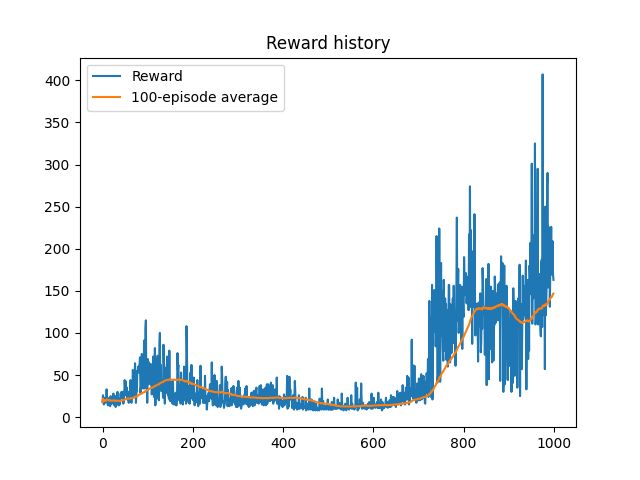
\includegraphics[width=0.7\columnwidth]{img/Figure_1_task_1a_cumulative_reward.png}
	\caption{Training performance using basic REINFORCE without baseline.}
	\label{fig:fig1}
\end{figure}

\begin{figure}[pht] 
	\centering  % Remember to centre the figure
    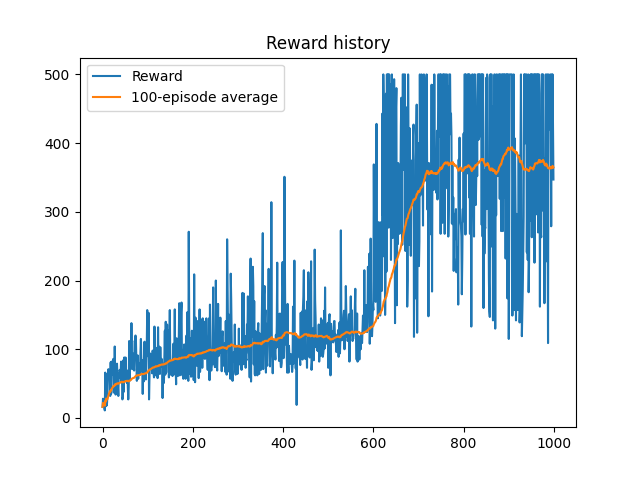
\includegraphics[width=0.8\columnwidth]{img/Figure_2_task_1b_cumulative_reward.png}
	\caption{Training performance using REINFORCE with a constant baseline $b = 20$.}
	\label{fig:fig2}
\end{figure}


\begin{figure}[phb] 
	\centering  % Remember to centre the figure
    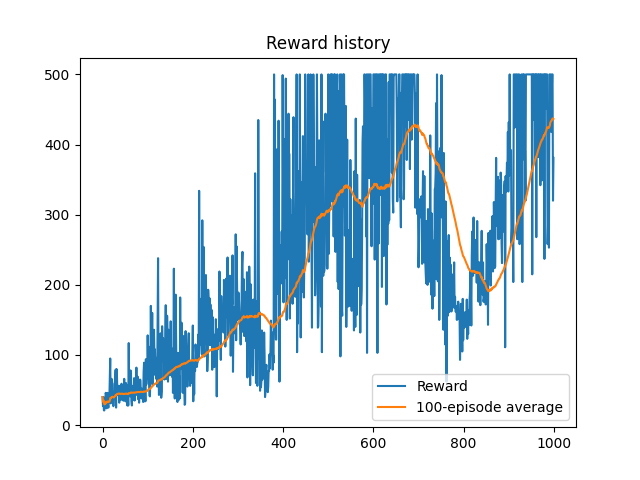
\includegraphics[width=0.8\columnwidth]{img/Figure_3_task_1c_cumulative_reward.png}
	\caption{Training performance using REINFORCE with discounted rewards normalized to zero mean and unit variance.}
	\label{fig:fig3}
\end{figure}


\pagebreak


\section*{Question 1.1}

How would you choose a good value for the baseline? \textbf{Justify your
answer.}
\newline

All the rewards are positive so subtracting a constant baseline (such as $b=20$ in case 1b) improves gradient calculation. The average of rewards is a good choice as a baseline. It may not be the optimum choice but it works well in practise (see Section 2.8 of Sutton's book).

\section*{Question 1.2}

How does the baseline affect the training, and \textbf{why?}
\newline

The baseline affects the variance of the update and thus the rate of convergence. Decreasing bias in policy gradient estimation produces less noisy gradient estimates because the variance of the estimator is decreased (Quiz).

\section*{Task 2}

The training performance plots for Task 2a and 2b are presented in Figures~\ref*{fig:fig4} 
and \ref*{fig:fig5}. REINFORCE with normalized discounted returns and the initial value $\sigma_0^2 = 100$ were used  
in both cases.

%\begin{itemize}
\begin{enumerate}[label=(\alph*)]
    \item exponentially decaying variance $\sigma^2 = \sigma_0^2 \cdot \operatorname{e}^{-c \cdot k}$ where $c = 5 \cdot 10^{−4}$ and $k$ is the number of episode, 
    \item variance learned as a parameter of the network
\end{enumerate}
%\end{itemize}

\noindent
Source files: cartpole.py, agent\_task2a.py, agent\_task2b.py


\begin{figure}[phb] 
	\centering  % Remember to centre the figure
    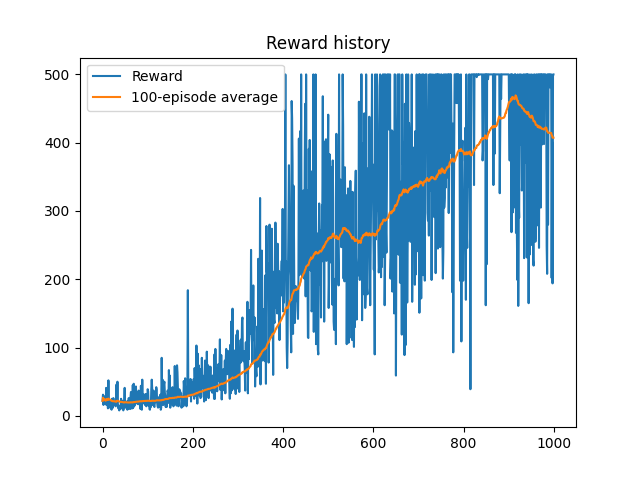
\includegraphics[width=0.8\columnwidth]{img/Figure_4_task_2a_cumulative_reward.png}
	\caption{Training performance using exponentially decaying variance.}
	\label{fig:fig4}
\end{figure}

\begin{figure}[pht] 
	\centering  % Remember to centre the figure
    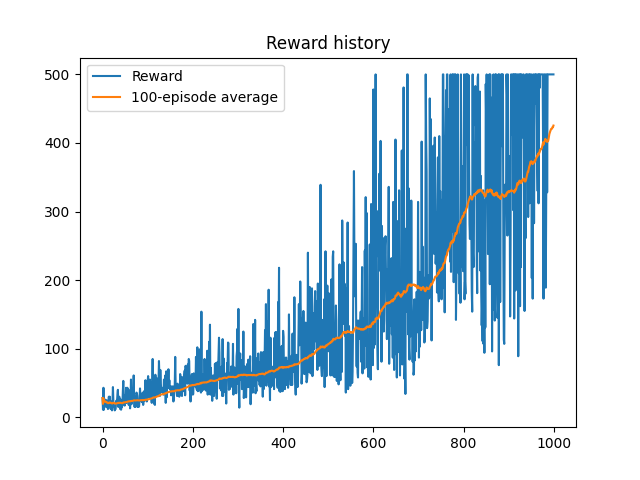
\includegraphics[width=0.8\columnwidth]{img/Figure_5_task_2b_cumulative_reward.png}
	\caption{Training performance using variance learned as a parameter of the network.}
	\label{fig:fig5}
\end{figure}

\pagebreak

\section*{Question 3.1}

Compare using a constant variance, as in Task 1, to using exponentially decaying variance and to learning variance during training. \textbf{Please explain} what the strong and weak sides of each of those approaches are.
\newline

The good point of using constant variance is, of course, simplicity. The weak sides are, e.g., slow convergence, especially when combined with unbounded rewards without normalization, as shown in Figure 1. If the constant variance is too small, training may not converge at all, and if the constant variance is very large, there may be large oscillations in training performance, as shown in Figure 3. 
\newline 

Both exponentially decaying variance and learning variance during training appear to allow faster convergence compared to constant variance and also stabilize the learning process and the training performance, as shown in Figures 4 and 5. The weak point, especially with learning variance during training, is the complexity of optimizing  hyperparameters (e.g., learning rate $\alpha$ and initializing parameters) because they can have a huge impact on the training results.


\section*{Question 3.2}

In case of learned variance, what’s the impact of initialization on the
training performance? \textbf{Please explain.}
\newline

As with other hyperparameters, initialization of the learned variance can have a major impact on the training performance. For example, if the initial variance is too small (e.g., $\sigma_0^2 = 1.0$), the training performance does not converge during 1000 episodes.


\section*{Question 4.1}

Could the method implemented in this exercise be \textbf{directly} used
with experience replay? \textbf{Why/why not?}
\newline 

No because the experience replay method requires an off-policy algorithm and the MC policy gradient - REINFORCE is an on-policy method.


\section*{Question 4.2}

Which steps of the algorithm would be problematic to perform with
experience replay, if any? \textbf{Explain your answer.}
\newline

We used an episodic version of REINFORCE that stored the action's outcome (i.e. states, action probabilities, rewards) and used it only at the end of the episode to update the policy through gradient calculation, while the experience replay method at each time step samples experiences from the replay memory and then uses them to update the learning process. 
\newline

The experience replay method also pulls unconnected experiences out of the replay memory to provide data for the next update, which requires an off-policy algorithm that does not need to be applied along connected trajectories (see Section 16.5 of Sutton's book).


\section*{Question 5.1}

What could go wrong when a model with an unbounded continuous
action space and a reward function like the one used here (+1 for survival) were to be used with
a physical system?
\newline

With unbounded returns, the variance of the unbounded continuous action space model may not converge at all during training.


\section*{Question 5.2}

How could the problems appearing in Question 5.1 be mitigated
without putting a hard limit on the actions? \textbf{Explain your answer.}
\newline

The easiest way is to subtract the baseline from the discounted rewards or otherwise normalize the discounted rewards (e.g., to zero mean and unit variance), as was done in Task 1 and 2.


\section*{Question 6}

Can policy gradient methods be used with discrete action spaces?
Why/why not? Which steps of the algorithm would be problematic to perform, 
if any? \textbf{Explain your answer.}
\newline

Yes, policy gradient methods can be used with discrete action spaces, such as soft-max policy with an exponential soft-max distribution (see slide 6 of Lecture 5).
\newline

In the REINFORCE algorithm, the policy estimator could  have been implemented using the Softmax function, which provides the probability estimates of the actions (that sum to 1.0). The action for each time step would have been randomly selected based on the probability estimates. Perhaps the calculation of the optimization term (=loss) would have been more complex because the selection of action\_probs is then based on action indexes. 





\bibliographystyle{ieeetr}
\bibliography{template}  % Modify template with your bibliography name
\end{document}
